% This is the Reed College LaTeX thesis template. Most of the work
% for the document class was done by Sam Noble (SN), as well as this
% template. Later comments etc. by Ben Salzberg (BTS). Additional
% restructuring and APA support by Jess Youngberg (JY).
% Your comments and suggestions are more than welcome; please email
% them to cus@reed.edu
%
% See http://web.reed.edu/cis/help/latex.html for help. There are a
% great bunch of help pages there, with notes on
% getting started, bibtex, etc. Go there and read it if you're not
% already familiar with LaTeX.
%
% Any line that starts with a percent symbol is a comment.
% They won't show up in the document, and are useful for notes
% to yourself and explaining commands.
% Commenting also removes a line from the document;
% very handy for troubleshooting problems. -BTS

% As far as I know, this follows the requirements laid out in
% the 2002-2003 Senior Handbook. Ask a librarian to check the
% document before binding. -SN

%%
%% Preamble
%%
% \documentclass{<something>} must begin each LaTeX document
\documentclass[12pt,twoside,openany]{reedthesis}
% Packages are extensions to the basic LaTeX functions. Whatever you
% want to typeset, there is probably a package out there for it.
% Chemistry (chemtex), screenplays, you name it.
% Check out CTAN to see: http://www.ctan.org/
%%

\usepackage{setspace}
\usepackage{graphicx,latexsym}
\usepackage{amsmath}
\usepackage{amssymb,amsthm}
\usepackage{longtable,booktabs,setspace, array}
\usepackage[hyphens]{url}
\usepackage{hyperref}
% Added by JLB
\usepackage{lineno} % line numbers
\linenumbers

\usepackage{lmodern}

\usepackage{float}
\floatplacement{figure}{h}

\usepackage{rotating}

\usepackage{natbib}
% Comment out the natbib line above and uncomment the following two lines to use the new
% biblatex-chicago style, for Chicago A. Also make some changes at the end where the
% bibliography is included.
% \usepackage{biblatex-chicago}
% \bibliography{thesis}


% Added by CII (Thanks, Hadley!)
% Use ref for internal links
\renewcommand{\hyperref}[2][???]{\autoref{#1}}
\def\chapterautorefname{Chapter}
\def\sectionautorefname{Section}
\def\subsectionautorefname{Subsection}
% End of CII addition

% Added by CII
\usepackage{caption}
\captionsetup{width=5in}
% End of CII addition

% \usepackage{times} % other fonts are available like times, bookman, charter, palatino

% Syntax highlighting #22

% To pass between YAML and LaTeX the dollar signs are added by CII
\title{Regime Detection Measures for the Practical Ecologist}
\author{Jessica L. Burnett}
% The month and year that you submit your FINAL draft TO THE LIBRARY
\date{2019}
% \division{}
\advisor{Craig R. Allen}
\department{School of Natural Resources}
\institution{University of Nebraska-Lincoln}
\degree{Doctor of Philosophy}
%If you have two advisors for some reason, you can use the following
% Uncommented out by CII
\altadvisor{Dirac Twidwell}
% End of CII addition

%%% Remember to use the correct department!
% if you're writing a thesis in an interdisciplinary major,
% uncomment the line below and change the text as appropriate.
% check the Senior Handbook if unsure.
%\thedivisionof{The Established Interdisciplinary Committee for}
% if you want the approval page to say "Approved for the Committee",
% uncomment the next line
%\approvedforthe{Committee}

% Added by CII
%%% Copied from knitr
%% maxwidth is the original width if it's less than linewidth
%% otherwise use linewidth (to make sure the graphics do not exceed the margin)
\makeatletter
\def\maxwidth{ %
  \ifdim\Gin@nat@width>\linewidth
    \linewidth
  \else
    \Gin@nat@width
  \fi
}
\makeatother

\renewcommand{\contentsname}{Table of Contents}
% End of CII addition

\setlength{\parskip}{0pt}

% Added by CII

\providecommand{\tightlist}{%
  \setlength{\itemsep}{0pt}\setlength{\parskip}{0pt}}

\Acknowledgements{

}

\Dedication{

}

\Preface{

}

\Abstract{

}

% End of CII addition
%%
%% End Preamble
%%
%
\begin{document}

% Everything below added by CII
  \maketitle

\frontmatter % this stuff will be roman-numbered
\pagestyle{empty} % this removes page numbers from the frontmatter

%

  \hypersetup{linkcolor=black}
  \setcounter{tocdepth}{2}
  \tableofcontents

  \listoftables

  \listoffigures


%
\mainmatter % here the regular arabic numbering starts
\pagestyle{fancyplain} % turns page numbering back on
\doublespacing{} % Trying to set spacing between lines in body
% \linespread{1.6} % Trying to set spacing between lines in body

\chapter{thesisdown::thesis\_gitbook:
default}\label{thesisdownthesis_gitbook-default}

Placeholder

Identifying abrupt changes in the structure and functioning of systems,
or system regime shifts, in ecological and social-ecological systems
leads to an understanding of relative and absolute system resilience.
Resilience is an emergent phenomenon of complex social-ecological
systems, and is the ability of a system to absorb disturbance without
reorganizing into a new state, or regime. Resilience science provides a
framework and methodology for quantitatively assessing the capacity of a
system to maintain its current trajectory (or to stay within a certain,
and often desirable regime). If and when a system's resilience is
exceeded, it crosses a threshold and enters into an alternate regime (or
undergoes a regime shift).\\
I will use Fisher Information to detect regime shifts in time and space
using avian community data obtained from the North American Breeding
Bird Survey within the area east of the Rockies and west of the
Mississippi River. Fisher Information is a technique that captures the
dynamic of a system, and this metric will be calculated about a suite of
bird species abundances aggregated to the route level for all possible
time periods. Transmutation (aggregation error) about inclusion or
exclusion of certain bird species, functional groups, and guilds will be
analyzed. Efforts have been made to develop early warning indicators of
regime shifts in ecosystems, however, for most ecosystems there is great
uncertainty in predicting the risk of a regime shift, regarding both
when and how long it will take to happen and if it can be recognized
early enough to be avoided when desired. We will complement the use of
Fisher Information with multiple discontinuity analyses about body mass
distributions at the route-level to achieve the aim of identifying
individual species that best serve as early-warning indicators of regime
shifts. For those species found on the edges of body mass aggregations,
we test the hypothesis that the background variance in their abundances
(on Breeding Bird Survey routes) will increase more than those not
observed at the edge of discontinuity aggregations. Identification of
early-warning indicators of regime shifts in ecological systems allows
management efforts to focus on a single or a small number of species
that inform us about ecosystem resilience and trajectory.\\
These methods transcend the primary objective of the Breeding Bird
Survey (to monitor population trends) and use this expansive dataset in
such a way that information about ecosystem order, trajectory, and
resilience emerge. Here, we utilize an expansive dataset (the Breeding
Bird Survey) to make broad-scale estimations and predictions about
ecosystem resilience, regime status and trajectory, and ecosystem
sustainability. Identification of regime shifts and early-warning
indicator species may afford us the ability to predict system regime
shifts in time.

\chapter*{Table of Definitions}\label{definitions}
\addcontentsline{toc}{chapter}{Table of Definitions}

Research surrounding regime shifts, threshold identification,
change-point detection, bifurcation theory, etc. is muddled with jargon.
Here, I provide a table of definitions (Table \ref{tab:glossary}) for
terms and concepts that may either be unfamiliar to the practical
ecologist, or may have multiple meanings among and within ecological
researchers and practitioners. With this table, I aim to both improve
the clarity of this dissertation \emph{and} highlight one potential
issue associated with regime detection methods in ecology: semantics.

\begingroup\fontsize{10}{12}\selectfont
\begin{longtable}{>{\raggedright\arraybackslash}p{8em}>{\raggedright\arraybackslash}p{25em}>{\raggedright\arraybackslash}p{6em}}
\caption{\label{tab:glossary}A table of definitions for terms, theories, and phrases often appearing in ecological regime shift literature.}\\
\toprule
\textbf{Term} & \textbf{Definition} & \textbf{Synonyms}\\
\midrule
\endfirsthead
\caption[]{\label{tab:glossary}A table of definitions for terms, theories, and phrases often appearing in ecological regime shift literature. \textit{(continued)}}\\
\toprule
\textbf{Term} & \textbf{Definition} & \textbf{Synonyms}\\
\midrule
\endhead
\
\endfoot
\bottomrule
\endlastfoot
Abrupt & A relative value of the speed and/or intensity of the change; the time period over which the regime shift occurs relative to the time observed (or expected to have been) in a particular state. & big, fast, quick, large\\
\textbf{Alternative Stable State} & \textbf{Controversially can be distilled as one of either: the number of unique stable configurations that a system can adopt (see Lewontin 1969), or the impacts that processes or pressures can have on a system's state (see May 1977).} & \textbf{}\\
Attractor & The set of values towards which a system tends regardless of its initial (starting) vaules. & \\
\textbf{Basin-Boundary Collision} & \textbf{The parameter values for a system that causes the system to shift between alternate attractors.} & \textbf{non-local bifurcation}\\
Catastrophe Theory & The study of abrupt changes within a dynamical system. & \\
\addlinespace
\textbf{Catastrophic Bifurcation} & \textbf{A relatively abrupt jump to an alternate attractor due to initial attractor.} & \textbf{}\\
Change-Point & See also 'Regime Shift'. A term often used in computer science, climatology, data science; represents the point at which a state changes its configuration. & \\
\textbf{Change-Point Detection} & \textbf{A change point method which does not require supervision; identifies potential change points without a priori potential change points.} & \textbf{}\\
Change-Point Estimation & A change point method which DOES require supervision; identifies potential change points when given a set of potential change points; well-developed in computer science, statistics, data mining, etc.; although well-developed, still lacks with giving statistical significance of change-points. & \\
\textbf{Chaos} & \textbf{A system with extreme sensitivity to initial conditions.} & \textbf{}\\
\addlinespace
Critical Slowing Down (CSD) & When the recovery rate (time to return) of a system decreases (approaches zero) as a system approaches a critical point (possibly a threshold or tipping point). A characteristic observed in some empirical systems data (e.g. nutrient loading in shallow lakes). & \\
\textbf{Degrees of Freedom} & \textbf{The number of system parameters or components which vary independently.} & \textbf{}\\
Domain of Attraction & The range of values around which a system fluctuates. & zone of fluctuation, basin of attraction, stable point, attractor\\
\textbf{Driver} & \textbf{A widespread anthropogenic source of change which leads to one or more pressures (e.g., land-use change).} & \textbf{}\\
Driver-Threshold Regime Shift & When a rapid change in external driver indcues a rapid change in ecosystem state. & \\
\addlinespace
\textbf{Dynamical System} & \textbf{A time-dependent system which can be described in state-space.} & \textbf{}\\
Dynamical Systems Theory & The study of complex systems theory; the study of time-dependent systems. & \\
\textbf{Equilibrium} & \textbf{The set of values around which a system revolves and does not change.} & \textbf{}\\
Exogeneous Process (Forcing, Driver) & An external process influencing the state of the dynamical system. & \\
\textbf{First-Order Stationarity} & \textbf{When the mean is constantant over the observations.} & \textbf{}\\
\addlinespace
Fold Bifurcation & This occurs when a stable point collides with an unstable point; when crossing a tipping point induces hysteresis. & \\
\textbf{Fractal Properties} & \textbf{A measurement of geometrical self-similarity; when a system has similar structure regardless of the scale of observation.} & \textbf{ergodic}\\
Hysteresis & A system which is state-dependent (e.g. magnets); when a tipping point or threshold is crossed such that the previous state cannot be achieved by reversing the conditions. & \\
\textbf{Leading Indicators} & \textbf{When the statistical properties of the fluctuations (of the data) approach a critical transition.} & \textbf{}\\
Lyapunov Exponent (and Stability & A value that conveys the average rate of trajectory divergence that is caused by an endogenous force; how quickly (if at all) a system will tend away from a stable point if it starts near the stable point. & \\
\addlinespace
\textbf{Measure Theory} & \textbf{The study of measures and measurement (e.g. volume, mass, time).} & \textbf{}\\
Moving (Sliding) Window Analysis & When a subsample of the data \$\$X\_t\$\$ is used in lieu of a single observation, \$\$x\_t\$\$. & \\
\textbf{Noise} & \textbf{Processes manifested in data which are unaccounted for; sometimes referred to as meaningless; random variability.} & \textbf{}\\
Non-Stationarity of the Mean Value & Infers that a trend or a periodicity is present in the time series. & \\
\textbf{Online} & \textbf{Real-time updating of model parameters, predictions, etc. (c.f. offline).} & \textbf{}\\
\addlinespace
Persistent & A relative value of the longevity of the observed change in values. & long-lasting\\
\textbf{Phase Space} & \textbf{A graphical representation of two or more trajectories where one axis is not time. In this representation an equilibrium is defined as a single point in the state space.} & \textbf{}\\
Prediction & A temporal forecast. Is intrinsic when a model and paramters are used to make forecast, is realized when the prediction becomes the actual state of the system. & \\
\textbf{Pressure} & \textbf{A perturbation which negatively influences a system, and can be defined as pulse, press, or monotonic.} & \textbf{}\\
Red Noise & Noise having zero mean, constant variance, and serial autocorrelation; autocorrelated random variability. & \\
\addlinespace
\textbf{Regime} & \textbf{A set of system values that define a particular system state. Not necessarily stable, but some state variables or outputs of the system remain relatively constant over a defined period of time.} & \textbf{}\\
Regime Shift & "abrupt" and "persistent" change in a system's structure or functioning. & \\
\textbf{Second-Order Stationarity} & \textbf{The nean is constant and the covariance is a function of a time lag, but not of time.} & \textbf{}\\
Self-Similarity & A system satisfied by  power-law scaling. & \\
\textbf{Stable Equilibrium} & \textbf{An equilibrium is stable when small perturbations do not induce change.} & \textbf{}\\
\addlinespace
State Space & The set of all possible configurations of a system. & \\
\textbf{State-Threshold Regime Shift} & \textbf{When a graduaal change in external driver induces a rapid change in ecosystem state (e.g,. System crosses a threshold).} & \textbf{}\\
Stationarity & When the probability density function of a system does not change with time. & \\
\textbf{Statistical Stationarity} & \textbf{A system with statistical properties unchanging over time. This concept extends to periodic stationarity for systems exhibiting periodic behavior.} & \textbf{}\\
Strange Attractor & An attractor which has fractal structure (an observable fractal dimension). & \\
\addlinespace
\textbf{Supervised Machine Learning} & \textbf{When classifiers are used to train the data a priori.} & \textbf{}\\
System State & The observed (current) instance of the system within a state space. & \\
\textbf{Threshold} & \textbf{A point where the system reacts to changing conditions.} & \textbf{}\\
Tipping Point & A point in a system's trajectory where a small change in an endogenous force induces a large change in sytem state or values; the point where a system can flip into an alternative state. & \\
\textbf{Trajectory} & \textbf{The path of an object or system through space-time.} & \textbf{orbit, path}\\
\addlinespace
Transient & A behavior or phenomenon which is responsive to intial (starting) conditions, or its effect declines over time. & \\
\textbf{Trend Smoothing} & \textbf{Local averaging of values such that the non-systematic components of the system are washed out.} & \textbf{}\\
Unstable Equilibrium & An equilibrium is unstable when small perturbations induce change. & \\
\textbf{Unsupervised Maain Learning} & \textbf{When no prior training of the data is required (i.e. no classifications necessary a priori) to classify it.} & \textbf{}\\
White Noise & Noise having zero mean, constant variance, and is not autocorrelated; uncorrelated random variability. & \\*
\end{longtable}
\endgroup{}

\chapter{Introduction}\label{intro}

Placeholder

\section{Forecasting abrupt changes in
ecology}\label{forecasting-abrupt-changes-in-ecology}

\section{Dissertation aims}\label{dissertation-aims}

\section{Dissertation structure}\label{dissertation-structure}

\subsection{Chapter overview}\label{chapter-overview}

\subsection{Accompanying software
(appendices)}\label{accompanying-software-appendices}

\chapter{A brief overview of ecological regime detection methods
methods}\label{rdmReview}

Placeholder

\section{Introduction}\label{introduction}

\section{Methods}\label{methods}

\subsection{Identifying candidate
articles}\label{identifying-candidate-articles}

\subsubsection{Web of Science}\label{web-of-science}

\subsubsection{Prior knowledge and snowball
method}\label{prior-knowledge-and-snowball-method}

\subsubsection{Google Scholar}\label{google-scholar}

\subsubsection{Additional filtering}\label{additional-filtering}

\section{Results}\label{results}

\subsection{Web of Science}\label{web-of-science-1}

\subsection{Google Scholar and prior
knowledge}\label{google-scholar-and-prior-knowledge}

\subsection{List of new methods}\label{list-of-new-methods}

\section{Discussion}\label{discussion}

\subsection{Barriers to identifying new regime detection
measures}\label{barriers-to-identifying-new-regime-detection-measures}

\subsection{Reducing the barriers to regime detection
measures}\label{reducing-the-barriers-to-regime-detection-measures}

\chapter{A guide to Fisher Information for Ecologists}\label{fiGuide}

Placeholder

\section{Abstract}\label{abstract}

\section{Introduction}\label{introduction-1}

\subsection{On Fisher Information}\label{on-fisher-information}

\subsection{Notation}\label{notation}

\subsection{Steps for calculating Fisher Information
(FI)}\label{steps-for-calculating-fisher-information-fi}

\subsection{Concepts behind the
calculations}\label{concepts-behind-the-calculations}

\subsubsection{\texorpdfstring{\textbf{Step 1. Probability of observing
the system in a particular state,
\(p(x)\)}}{Step 1. Probability of observing the system in a particular state, p(x)}}\label{step-1.-probability-of-observing-the-system-in-a-particular-state-px}

\subsubsection{\texorpdfstring{\textbf{Step 2.} Distance traveled by the
system,
\(s\)}{Step 2. Distance traveled by the system, s}}\label{step-2.-distance-traveled-by-the-system-s}

\subsubsection{\texorpdfstring{\textbf{Step 3.} \(p(s)\) as a function
of the rate of change of
\(s\)}{Step 3. p(s) as a function of the rate of change of s}}\label{step-3.-ps-as-a-function-of-the-rate-of-change-of-s}

\subsubsection{\texorpdfstring{\textbf{Step 4.} Calculate the
derivatives-based Fisher
Information}{Step 4. Calculate the derivatives-based Fisher Information}}\label{step-4.-calculate-the-derivatives-based-fisher-information}

\section{Case Study}\label{case-study}

\section{Conclusions}\label{conclusions}

\section{Acknowledgements}\label{acknowledgements}

\chapter{An application of Fisher Information to spatially-explicit
avian community data}\label{fisherSpatial}

Placeholder

\section{Introduction}\label{introduction-2}

\section{Data and methods}\label{data-and-methods}

\subsection{Data: North American breeding bird
communities}\label{data-north-american-breeding-bird-communities}

\subsection{Study area}\label{study-area}

\subsubsection{Focal military base}\label{focal-military-base}

\subsubsection{Spatial sampling grid}\label{spatial-sampling-grid}

\subsection{Calculating Fisher Information
(FI)}\label{calculating-fisher-information-fi}

\subsection{Interpreting and comparing Fisher Information across spatial
transects}\label{interpreting-and-comparing-fisher-information-across-spatial-transects}

\subsubsection{Interpreting Fisher Information
values}\label{interpreting-fisher-information-values}

\subsubsection{Interpolating results across spatial
transects}\label{interpolating-results-across-spatial-transects}

\subsubsection{Spatial correlation of Fisher
Information}\label{spatial-correlation-of-fisher-information}

\section{Results}\label{results-1}

\subsection{Fisher Information across spatial
transects}\label{fisher-information-across-spatial-transects}

\subsection{Spatial correlation of Fisher
Information}\label{spatial-correlation-of-fisher-information-1}

\section{Discussion}\label{discussion-1}

\subsection{Efficacy of Fisher Information as a spatial
RDM}\label{efficacy-of-fisher-information-as-a-spatial-rdm}

\chapter{\texorpdfstring{Velocity (\emph{v}): using rate-of-change of a
system's trajectory to identify abrupt
changes}{Velocity (v): using rate-of-change of a system's trajectory to identify abrupt changes}}\label{velocity}

Placeholder

\section{Introduction}\label{introduction-3}

\section{Data and Methods}\label{data-and-methods-1}

\subsection{Theoretical system example: two-species time
series}\label{theoretical-system-example-two-species-time-series}

\subsection{\texorpdfstring{Steps for calculating system velocity,
\emph{v}}{Steps for calculating system velocity, v}}\label{steps-for-calculating-system-velocity-v}

\subsubsection{\texorpdfstring{Step 1:
\(\Delta x_i\)}{Step 1: \textbackslash{}Delta x\_i}}\label{step-1-delta-x_i}

\subsubsection{\texorpdfstring{Step 2:
\(\sqrt(\sum_i^N\Delta x_1^2)\)}{Step 2: \textbackslash{}sqrt(\textbackslash{}sum\_i\^{}N\textbackslash{}Delta x\_1\^{}2)}}\label{step-2-sqrtsum_indelta-x_12}

\subsubsection{\texorpdfstring{Step 3: Use Pythagorean theorem to
isolate
\(s\)}{Step 3: Use Pythagorean theorem to isolate s}}\label{step-3-use-pythagorean-theorem-to-isolate-s}

\subsubsection{\texorpdfstring{Step 4: Calculate velocity, \(v\) (or
\(\frac {\Delta s}{\Delta t}\))}{Step 4: Calculate velocity, v (or \textbackslash{}frac \{\textbackslash{}Delta s\}\{\textbackslash{}Delta t\})}}\label{step-4-calculate-velocity-v-or-frac-delta-sdelta-t}

\subsection{\texorpdfstring{Velocity \emph{v} performance under varying
mean and variance in the toy
system}{Velocity v performance under varying mean and variance in the toy system}}\label{velocity-v-performance-under-varying-mean-and-variance-in-the-toy-system}

\subsubsection{Varying post-shift mean}\label{varying-post-shift-mean}

\subsubsection{Varying post-shift
variance}\label{varying-post-shift-variance}

\subsubsection{\texorpdfstring{Smoothing the data prior to calculating
\emph{v}}{Smoothing the data prior to calculating v}}\label{smoothing-the-data-prior-to-calculating-v}

\subsection{Performance on empirical data: paleodiatom community
example}\label{performance-on-empirical-data-paleodiatom-community-example}

\section{Discussion}\label{discussion-2}

\section{Supplementary Materials}\label{supplementary-materials}

\chapter{Data Quality Impacts on Regime Detection
Measures}\label{resampling}

\textbf{SEE IIASA REPORT} (.doc)

\section{Introduction}\label{introduction-4}

Ecological systems have many unpredictable and variably interacting
components (Jørgensen et al. 2011). Methods for analyzing these complex
systems, e.g.~Dynamic Bayesian Networks, network models, and food webs
are designed to handle these complexities, yet require data- and
knowledge-intensive models. Although ecological data collection and data
management techniques are improving (La Sorte et al. 2018), the
aforementioned approaches to modeling and understanding complex system
are often infeasible in ecosystem research and management (Clements et
al. 2015).

A growing concern with anthropogenic impacts on the environment has
increased the demand for mathematical and statistical techniques that
capture these dynamics. These often undesirable changes in the structure
or functioning of ecological systems are often referred to as ``regime
shifts'', ``regime changes'', ``state change'', ``abrupt change'', etc.
(Andersen et al. 2009) . A yet-unattained goal of ecological research
and management is to reach a point where these methods can predict
impending regime shifts in real-time and with high confidence. Ideally,
ecological regime shift detection methods (hereafter, regime detection
measures) would require little knowledge of the intrinsic drivers of the
system, and the users of the method would not be required to know if and
where a regime shift occurred in the data.

Despite the suite of regime detection measures in the environmental and
ecological research literatures, they are not used in ecological
management. We can describe the current state of regime detection
measures as being either system--specific (i.e., the method is not
widely applicable or generalizable across systems) or not. Methods of
the latter type are convenient in that they can be applied across
various system and data types, but the results of these analyses require
some degree of subjective interpretation (Clements and Ozgul 2018; c.f.
Batt et al. 2013). Efforts to develop and/or improve regime detection
measures that can handle these biases will aid the advance of regime
detection measures research and application.

Current efforts to improve regime detection measures may be stunted by
the lack of application beyond simple and/or theoretical (toy) systems
data. Like most statistical and mathematical approaches, the evolution
of many regime detection measures begins with application to theoretical
data, followed by application to empirical data. Current applications of
regime detection measures to empirical, ecological data are largely
limited to data describing populations (e.g., Anderson and Piatt 1999,
Alheit et al. 2005, deYoung et al. 2008), climatic, marine (e.g.,
Lipizer et al. n.d., Nicholls 2011), and Paleolithic regime shifts
(Spanbauer et al. 2014, Yang et al. 2017, Kong et al. 2017), with few
applications terrestrial data (c.f. Bahlai et al. 2015, Sundstrom et al.
2017). Although testing the performance and inference boundaries of
theoretical and simple systems is important, they are of little use to
ecosystem managers if they are not proven to be easily and reliably
applicable to their system. Additionally, regime detection measures
should be capable of handling diverse and often noisy field data.

Ecological systems data is not only expensive to capture, but are often
difficult to perfectly capture due to the large process and observation
errors. The variability resulting from imperfect observation influences
data quality and quantity, sometimes limiting the potential numerical
tools used to identify trends and changes in the system in question
(Thrush et al. 2009). Some methods, new and old, are proposed in the
literature as regime detection measures which are capable of handling
data limitation and quality issues inherent in ecological data and
require few subjective decisions for choosing state variables and
interpreting results. For example, variable reduction techniques,
e.g.~principal components analysis (Rodionov 2005, Andersen et al. 2009,
Reid et al. 2016) and clustering algorithms (Weijerman et al. 2005,
Weissmann and Shnerb 2016), an index of variance (Brock and Carpenter
2006) and Fisher Information (Cabezas and Fath 2002, Fath and Cabezas
2004, Karunanithi et al. 2008) were introduced as methods which collapse
the system into a single indicator of ecological regime shifts. Although
these methods have been tested on empirical ecological systems data,
their robustness to empirical data quality and quantity have yet to be
examined.

In this Chapter I examine the influence of observation and process
errors on the inference obtained from select multivariable regime
detection measures. There are two major objectives: 1. Identify the
effects of data quality on regime detection measure inference. 1.
Identify the effects of data quantity on regime detection measure
inference. 1. Explore the relative performance of velocity {[}described
in Chapter \ref{velocity}{]} to the abovementioned methods under
multiple scenarios.

This Chapter provides baseline relative performance estimates of select,
multivariable regime detection measures under various scenarios of data
quality and quantity. The results from this Chapter inform the practical
ecologist of the potential limitations to consider when applying these
regime detection measures to their data, and has potential to inform the
data collection process. Additionally, the software accompanying this
Chapter (soon to be an R Package) allows the end user to implement these
methods on their data.

\section{Data and Methodology}\label{data-and-methodology}

\subsection{Study system and data}\label{study-system-and-data}

I used paleodiatom time series from a freshwater system in North America
(Foy Lake, present day Montana) that apparently underwent a rapid shift
in algal community dynamics at multiple periods in time. This datum
comprises a single soil core sample, from which the relative abundances
of 109 diatom species were identified at 768 observations (time points)
over \(\approx7,00\) years {[}\ref{fig:origDat}{]}. Althouh the soil
core was sampled at regular distances, the soil accumulation process is
not necessarily linear over time, resulting in irregularly-sampled
observations (i.e., time elapsed between sampling points differs varies;
see \ref{fig:timeElapsed}). This datum was published in ({\textbf{???}})
and can be downloaded at the publisher's website.
\begin{figure}

{\centering 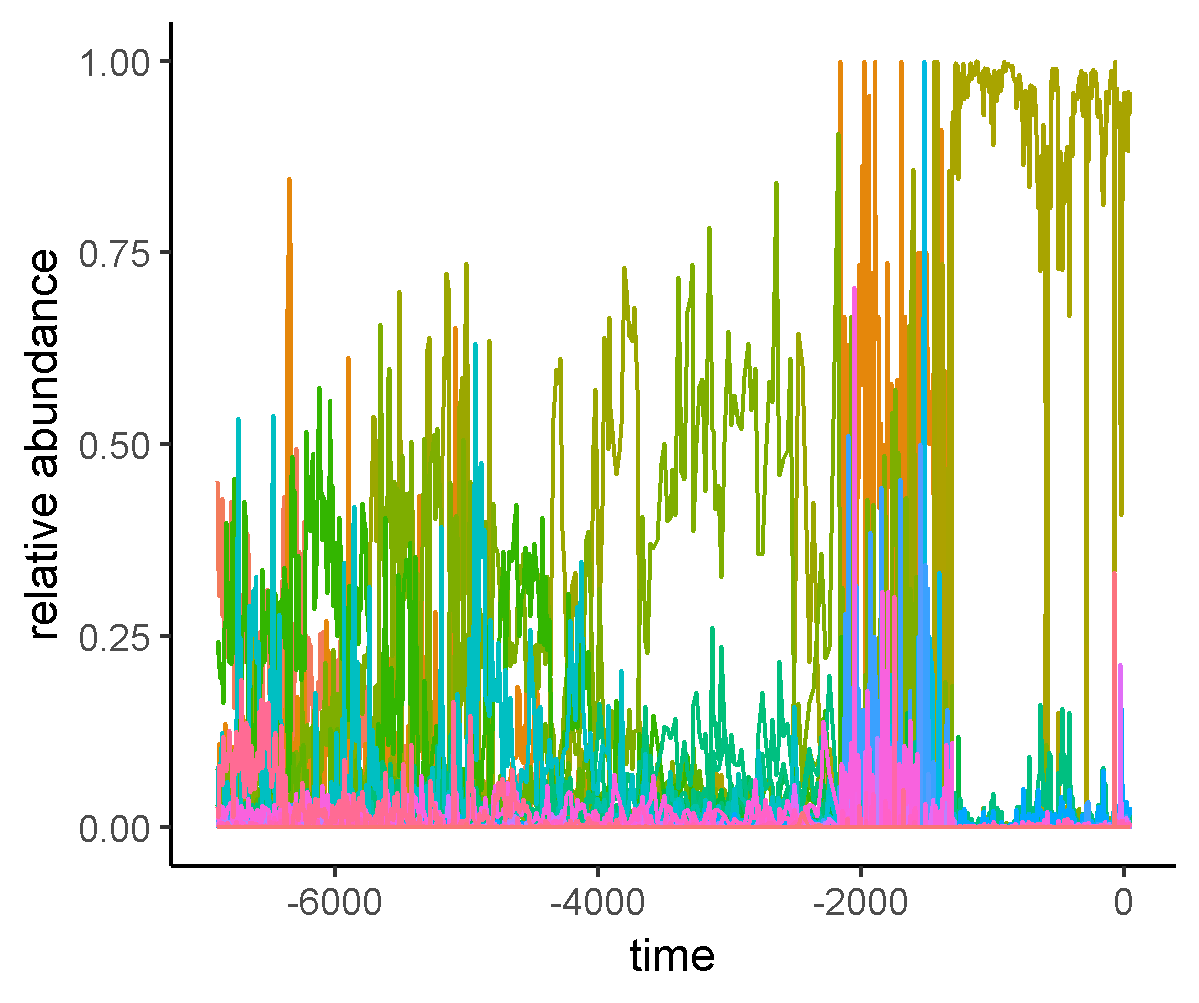
\includegraphics[width=0.85\linewidth]{./chapterFiles/resampling/figsCalledInDiss/origDataRelAbundance} 

}

\caption{Relative abundances of the diatom species in Foy Lake over the time period.}\label{fig:origDat}
\end{figure}
\begin{figure}

{\centering 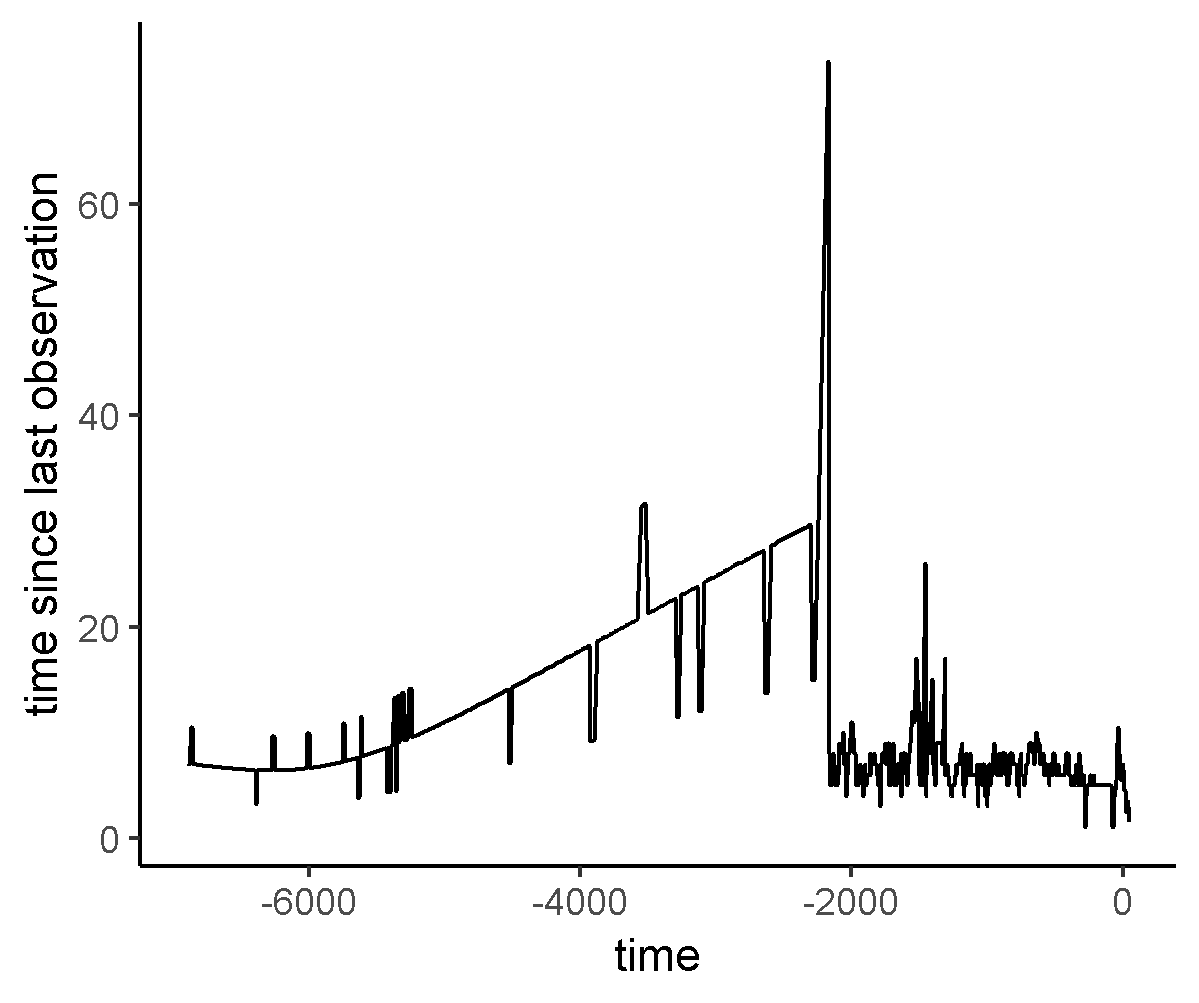
\includegraphics[width=0.85\linewidth]{./chapterFiles/resampling/figsCalledInDiss/timeElapsed} 

}

\caption{The amount of time elapsed between observations.}\label{fig:timeElapsed}
\end{figure}
\subsection{Regime detection measures}\label{regime-detection-measures}

Fewer model-free regime detection metrics exist than do model-based
metrics {[}Chapter \ref{rdmReview}{]} and of these, only a few are
suggested for handling multivariable data. Here, I examine the regime
detection metrics that are model-free and can handle multivariable data:
velocity {[}Chapter \ref{velocity}{]}, the Variance Index (Brock \&
Carpenter, 2006) and Fisher Information. These methods and the primary
sources are described below.

\subsubsection{\texorpdfstring{Velocity
(\(v\))}{Velocity (v)}}\label{velocity-v}

In Chapter \ref{velocity}, I describe a new method, \textbf{velocity},
\(v\), as a potential dimension reduction and regime detection method.
First introduced in by Fath, Cabezas, \& Pawlowski (2003) as one of
multiple steps in calculating their variant of Fisher Information,
velocity calculates the cumulative sum of the square root of the sum of
the squared change in all state variables over a period of time {[}Eq.
\eqref{eq:velocityEq}{]}. Steps for calculating this metric are described
in detail in Chapters \ref{fiGuide} and \ref{velocity}.
\begin{equation}
\begin{array}{rcr}
\Delta s_i = \sqrt{\sum_{j=1}^{n} (x_{i,j} -x_{i-1, j})^2}
s_k =  \sum_{i=2}^{k}\Delta{s_i}
2\leq k \leq n
v =\frac{\Delta s}{\Delta t}  
\end{array}
\label{eq:velocityEq}
\end{equation}
\subsubsection{Variance Index}\label{variance-index}

The Variance Index was introduced by Brock \& Carpenter (2006), and is
simply defined asthe maximum eigenvalue of the covariance matrix of the
system over some period (window) of time. The Variance Index (also
called Variance Indicator) was originally applied to a modelled system
(Brock \& Carpenter, 2006), and has since been applied to empirical data
({\textbf{???}}, {\textbf{???}}). Although rising variance has been
useful in many real systems (van Nes and Scheffer 2003, Brock et al.
2006, Carpenter and Brock 2006), the Variance Index, which is intended
for multivariate data, appears most useful when the system exhibits a
discontinuous regime shift (Brock \& Carpenter, 2006).

\subsubsection{Fisher Information}\label{fisher-information}

In Chapter \ref{fiGuide}, I describe Fisher Information in detail {[}see
Eq. \eqref{eq:fiDerivs}{]}. Fisher Information (\(I\)) is essentially
calculated as the area under the curve of the acceleration to the fourth
degree (\(s''^4\)) divided by the squared velocity {[}\(s'^2\); also
referred to as \(v\) in Chapter \ref{velocity} and in the next
section{]} of the distance travelled by the system, \(s\) over some
period of time (\(T\)), and is given in the following equation
{[}\eqref{eq:fiDerivs2}{]}:
\begin{equation}   
    I = \frac{1}{T} \int_0^T dt\left[\frac{s''^2}{s'^4}\right]^2 \\  
  \label{eq:fiDerivs2}  
\end{equation}
\subsubsection{Calculating Fisher Information and Variance Index using
moving window
analysis}\label{calculating-fisher-information-and-variance-index-using-moving-window-analysis}

Unlike \(velocity\), the Variance Index and Fisher Information are
calculated using moving window analysis. That is, over the entire time
series, \(T^*\), these metrics are calculated within multiple windows of
time, \(T\). In this approach, all state variables, \(x_i\), are used to
inform the calculations (of Variance Index and Fisher Information) over
a time interval, \(T\), where \(T\) is the length in {[}time{]} units of
the time interval and satisfies the following conditions: \(T < T^*\)
and \(2\leq T < (T^*-1)\). If \(T = T^*-1\), then only a single value of
the metrics will be calculated for entire time series, which does not
allow for any estimate of change.

When using these metrics in the context of identifying abrupt changes in
ecological systems data across \(T*\), it is ideal the value of \(T\)
meets the following conditions: \(3 < T \ll T^*-1\). The length of a
time window dictates the number of calculations one can obtain over
\(T^*\), such that the number of potential metric calulations increases
as \(\frac{T}{\ T^*}\) decreases. Previous applications of moving window
analyses to calculate Fisher Information found that at least eight
observations (time points) should be used.

An additional parameter is required when conducting moving window
analyses: the amount of time points by which the window advances. In
order to maximize the data, I force the window to advance at a rate of
one time unit. However, it is important to note that because these data
are not sampled annually and the because the window always advances by a
single time unit, the number of observations included in each
calculation will not be the same. If fewer than 5 observations are in a
window, I did not calculate metrics, advancing the window forward.

I assigned the calcuated values of Fisher Information and Variance Index
within each moving window to the \textbf{end} (last time unit) of the
moving window. I temporal analyses, assigning the value to any other
point in time (e.g., the beginning or the middle) muddles the
interpretation of the metric over \(T^*\).

\section{Results}\label{results-2}

\section{Discussion}\label{discussion-3}

\section{Ackowledgements}\label{ackowledgements}

This study was conceptualized at the International Institute for Applied
Systems Analysis (IIASA) as part of the Young Scholars Summer Program in
2018. I thank my IIASA program supervisors, Drs. Brian Fath and Elena
Rovenskaya, for advisement during this period and for comments on an
earlier version of this chapter.

\chapter{Discontinuity chapter under construction}\label{discontinuity}

\section{Introduction}\label{introduction-5}

\section{Data and Methods}\label{data-and-methods-2}

\section{Results}\label{results-3}

\section{Conclusions}\label{conclusions-1}

\chapter{Conclusions}\label{conclusions}

Placeholder

\section{Method mining regime detection
methods}\label{method-mining-regime-detection-methods}

\section{Ecological data are noisy}\label{ecological-data-are-noisy}

\section{Data collection and munging biases and limits
findings}\label{data-collection-and-munging-biases-and-limits-findings}

\section{Common Limitations of Regime Detection
Measures}\label{common-limitations-of-regime-detection-measures}

\section{Specific synthesis of chapter
results}\label{specific-synthesis-of-chapter-results}

\chapter*{Appendix A: R package
regimeDetectionMeasures}\label{regimeDetectionMeasures}
\addcontentsline{toc}{chapter}{Appendix A: R package
regimeDetectionMeasures}

Placeholder

\section{Measures/metrics calculated}\label{measuresmetrics-calculated}

\section{Example analysis}\label{example-analysis}

\chapter*{Appendix B: R package bbsRDM}\label{bbsRDM}
\addcontentsline{toc}{chapter}{Appendix B: R package bbsRDM}

Placeholder

\chapter*{References}\label{references}
\addcontentsline{toc}{chapter}{References}

Placeholder

\hypertarget{refs}{}
\hypertarget{ref-brock_variance_2006}{}
Brock, W., \& Carpenter, S. (2006). Variance as a Leading Indicator of
Regime Shift in Ecosystem Services. \emph{Ecology and Society},
\emph{11}(2). \url{http://doi.org/10.5751/ES-01777-110209}

\hypertarget{ref-fath_regime_2003}{}
Fath, B. D., Cabezas, H., \& Pawlowski, C. W. (2003). Regime changes in
ecological systems: An information theory approach. \emph{Journal of
Theoretical Biology}, \emph{222}(4), 517--530.
\url{http://doi.org/10.1016/S0022-5193(03)00067-5}


\end{document}
